\chapter{Game Tags for Topical Video Search}\label{chap:topicir-filter}
\begin{quotation}
\noindent
In this chapter we continue our investigation of the usefulness of the user tags for search. Particularly, our aim is to evaluate the performance of user tags for retrieval of videos that are about a given topic i.e. \textit{topical search}. To this end, we will reuse the same methodology as in Chap. \ref{chap:ecir}, namely \textit{quantitative system evaluation} \cite{vorhees}. The results presented bellow demonstrate that raw, unprocessed game tags are not well suited for retrieving video fragments based on topic. While the search recall is satisfactory, the search precision leaves much to be desired. This is mainly caused by the presence of game tags which are not valid topical annotations. Thus, the second aim of this work is to characterize the quality of the user tags as topical annotation and to detect and filter out the non-topical ones. We explore several features of the tags which could serve as an indication of their quality as topical descriptors. Our results show that after filtering, game tags can emulate the retrieval performance of a baseline system that utilizes manually crafted metadata for search. An important consequence of this finding is that tagging games can provide a cost-effective alternative in situations when manual annotation by professionals is too costly.

This chapter was accepted and will be published as ``Topical Video Search: Analysing Video Concept Annotation through Crowdsourcing Games" in the International Journal of Human Computation. It is co-authored with Michiel Hildebrand, Jacco van Ossenbruggen, Lora Aroyo, and Guus Schreiber.


\end{quotation}

\section{Introduction}

In the past decade audio-visual (AV) content collections have been undergoing a transformation from archives of analogue materials to very large stores of digital data accessible online\footnote{An excellent example is PrestoPRIME, \url{http://www.prestoprime.org/}, which was an European Union funded project about digitisation and preservation of the AV heritage. The consortium included the major national AV archives in Europe.}.  As the AV collection items become accessible to the wider internet audience the lack of adequate annotations is highlighted: users cannot find what they are looking for because annotations are either not present or too expert-centric --- created from the perspective of the catalogers \cite{johan-book-chap}. Video tagging games are an attempt to alleviate this problem. By engaging the internet community to tag their videos, the AV collection owners can benefit in at least two important ways. First, there is a clear cost-benefit, collecting annotations in this way is usually cheaper than using professional documentalists. Second, the game tags can help bridge the \textit{terminological gap} in search if the \textit{searchers} and \textit{annotators} originate from the same community and use similar terminology when searching and tagging. 

One of the most successful ongoing online video tagging games is \textit{Waisda?}.
The game was launched in 2009 by the Netherlands Institute for Sound and Vision (S\&V), one of the largest AV archives in Europe\footnote{S\&V manages and preserves over 70\% of the Dutch AV heritage. The collection contains more than 750.000 hours of television, radio, music and film from the beginning in 1898 until today.}.
The first pilot of the game run until January 2010 and produced over 420,000 user tags. Considering the acquired experience and insights, S\&V launched a second version of the game (see Chapter \ref{chap:waisda} for more details) which features several improvements, albeit the basic idea of the temporal tag agreement is preserved.

%\textit{Waisda?} is a multi-player game where players describe streaming video by entering tags and score points based on temporal tag agreement. The underlying assumption is that tags are faithful descriptions of the videos when entered independently by at least two players within a given time-frame.The first pilot of the game run until January 2010 and produced over 420,000 user tags. The analyses of the collected tags \cite{kcap} and user evaluations suggested potential areas of improvement. Considering the acquired experience and insights, S\&V launched a second version of the game\footnote{The game is deployed online and can be accessed at \url{http://woordentikkertje.manbijthond.nl/}. The source code is published as open-source under the GPL licence and can be downloaded from \url{https://github.com/beeldengeluid/waisda}.} which features several improvements, albeit the basic idea of the temporal tag agreement is preserved. 
%Figure \ref{filter:fig:game} shows the game page of \textit{Waisda?}. It contains a video player and below it a text-entry field. When the player enters the game page the video automatically starts playing, the text-entry field receives focus, and the player can start entering tags. The right side of the page contains the score board. It consists of the current score of the player, the current rank and a listing with all tags entered by the player. The tags are displayed with their score and an icon indicating the tag type (person, location etc.).
%\begin{figure}
%\centering
%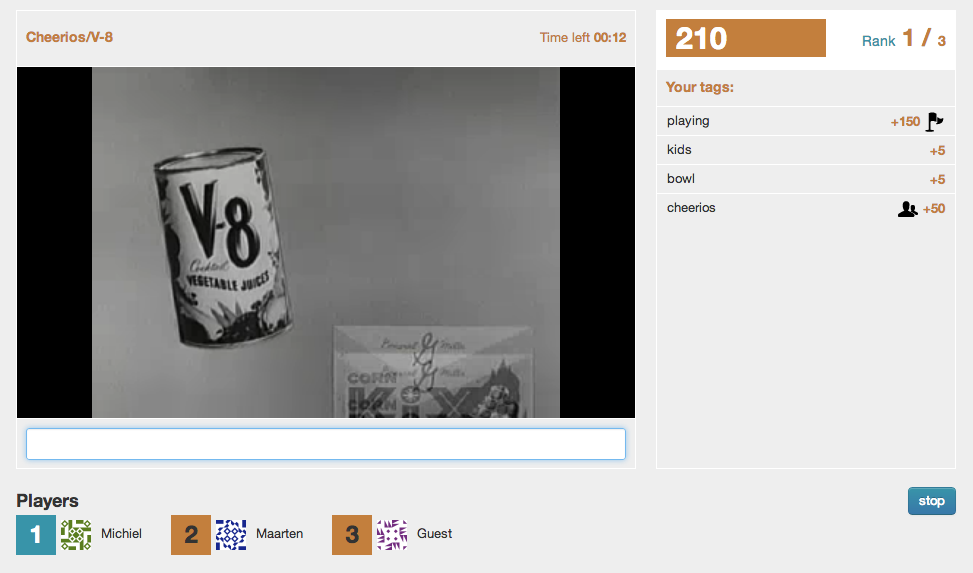
\includegraphics[scale=.35]{game.png}
%\caption{Screenshot of the \textit{Waisda?} game page with public domain video clip from Preligner Archives.}
%\label{filter:fig:game}
%\end{figure}

The second version of \textit{Waisda?}\footnote{At the time of writing the second version of the game has been discontinued. S\&V is deploying (still under development) a third installment of the game available at \url{http://waisda.beeldengeluid.nl/}. S\&V intends to integrate \textit{Waisda?} more tightly in their internal workflows and to use it to collect tags for the items in their online collection \url{http://in.beeldengeluid.nl/}.} is a mature, production-grade, customizible GWAP with diverse usage. 
It is included\footnote{\url{http://labs.europeana.eu/apps/waisda-floss}} as a showcase in the Europeana\footnote{Europeana is an internet portal that provides multi-lingual access to millions of books, paintings, films, and archival records that are part of the European cultural heritage. More than 2,000 institutions across Europe have contributed to the project.} internet portal. \textit{Waisda?} has also been deployed and incorporated in Spotvogel\footnote{\textit{Spotvogel} (\url{http://spotvogel.vroegevogels.vara.nl/}) which translates to \textit{mocking bird} from Dutch, was a \textit{Waisda?} deployment by the Dutch broadcaster VARA (\url{http://www.vara.nl/}) and the S\&V institute with the aim of collecting user tags for the footage from the Dutch television program \textit{Vroege Vogels} (\url{http://vroegevogels.vara.nl/}). The game run for 6 months in 2013 and was nominated for Dutch Game Awards 2013 \url{http://www.dutchgameawards.nl/2013/spotvogel/}, note that the link is in Dutch.}. In the former the internet users tag archival footage from the European cultural heritage and in the latter they identify occurrences of wildlife in footage. These are two relatively different domains yet \textit{Waisda?} was fitted to them seamlessly. This is due to the simple design of the game and the unconstrained way the tags are entered --- the players get a small set of instructions and then are free to enter whatever they please. This is a double-edged sword. On the one hand, the entry barrier for the players is low and the target audience is wide as no specific skills are needed. On the other hand, the open-ended way the tags are entered may be overwhelming in the fast-pased setting of the game and players may succumb to entering low quality tags which lack descriptive power just to reach consensus with other players and win points. In this study we perform a qualitative analysis to investigate this issue.

The cost-effectiveness of \textit{Waisda?} versus manual annotation by professionals comes with a caveat: successful deployment of a GWAP is no small feat. Attracting new players and keeping them engaged over time is vital for success and requires continuous publicising efforts. The empirical evidence collected from both \textit{Waisda?} pilots supports this claim. On both occasions the bulk of the tags was accumulated during periods when there was an active campaign for promoting the game. Targeting the fanbase of the TV series via various channels (e.g. TV series website, social media, etc.) has proved to be a successful strategy for attracting new players. Player's engagement is sustained with in-game mechanisms such as leaderboards to honour the best players and motivate the others, and with time-limited contests offering awards for the top performers. Planning and executing activities like these is certainly costly, however in the case where the growth rate of AV collections is ever increasing, these costs will be outweighed by the costs of manual annotation. This is one of the lessons learned from the \textit{Waisda?} project.


The second version of the game has amassed more than 710,000 user tags. The number of unique tags is 71,448 and each of the top five most-tagged videos has more than 3,600 tags ascribed to it which amounts to an average tag density of more than 13 tags per second. This is a substantially higher number than the number of tags assigned by professional catalogers, typically 10-20 tags per video. However, are all these user tags of any use? Does this overwhelming quantity implies quality? In Chapter \ref{chap:ecir} we demonstrated that the \textit{Waisda?} tags can indeed be successfully exploited for retrieving video fragments that feature \textit{visual appearances} of objects of interest (persons, objects, etc.) \cite{ecir}. Our results showed that \textit{Waisda?} tags excel at this kind of \textit{visual instance search}, outperforming the closed captions and annotations created by professionals. 

In this study we wish to understand whether the fast pace of \textit{Waisda?} forces players to have tunnel vision about the content of the video and tag predominately non-topical aspects.
Previous analysis performed by a senior cataloger from S\&V ruled the game tags to be limited in scope, referring mainly to things seen or heard on the screen \cite{waisda-lotte}.
However, we hypothesize that players do describe topics and topical tags are present albeit buried under the myriad of non-topical tags. The first research question, therefore is
\begin{itemize}
\item[RQ1] Do players enter tags which describe the topics of the videos?
\end{itemize}
In the context of topical video search, the presence of non-topical tags, which do not refer to the topics covered in the video, can lead to false positives. For example, if a video $v$ has a tag $t$ ascribed to it and $t$ does not refer to the topics covered in $v$. If a searcher is interested in videos that are about $t$ and uses $t$ as a search term the video $v$ will be incorrectly retrieved. Thus, it is important to know whether a tag is non-topical and ignore it in the retrieval process to eliminate its negative influence on the search results. Our second research question, therefore is
\begin{itemize}
\item[RQ2] Can the access to videos based on topic be improved by detecting and filtering out the non-topical game tags?
\end{itemize}

The rest of the chapter is structured as follows. In Section \ref{sec:topicir-filter:relatedwork} we discuss related work. Section \ref{sec:topicir-filter:approach} outlines our approach. In Section \ref{sec:topicir-filter:video-metadata-collection} and \ref{sec:topicir-filter:eval-ds} we describe the collection of video fragments and the evaluation dataset, respectively. Section \ref{sec:topicir-filter:all-tags} presents the findings with respect to the effectiveness of the user tags for topical search. This sets the baseline for the remainder of the study. In Section \ref{sec:topicir-filter:filtering} we outline a number of tag filters and evaluate their effectiveness for eliminating non-topical tags. Section \ref{sec:topicir-filter:con} presents the conclusions from the study.

\section{Related Work}\label{sec:topicir-filter:relatedwork}
\paragraph{User annotations for search.} Search based on user-generated metadata, in particular folksonomies, has been studied before. Morrison compared web search performance of folksonomies from social bookmarking web sites against search engines and subject directories \cite{morison}, showing that search engines had the highest precision and recall rates. Folksonomies, however, performed surprisingly well. In fact, user tags show promise to alleviate the vocabulary mismatch problem for search: bridging the gap between user queries and metadata used for retrieval \cite{vocprob}. Indeed, Geisler and Burns state that YouTube tags provide added value for search, because 66\% of them do not appear in  other metadata \cite{youtube}. Heymann et al. investigated a large-scale sample of forty million bookmarks from the social bookmarking site del.icio.us and found that in 20\% of the cases user tags do not occur in the page text, backlink page text, or forward link page text of the pages they annotate. Studies in \cite{Bischoff:2010:BGT:1833903.1834001,Halvey:2007:AOV:1286240.1286301,journals/jasis/Rorissa10,Yanbe:2007:SBE:1255175.1255198} investigate this phenomenon across multiple domains and multimedia resource types and identify the gaps between the tag space and the querying vocabulary. The common conclusion is that user tags can improve search by bridging the vocabulary gap. 

Studies reported in \cite{Bischoff:2008:TUS:1458082.1458112,Sun:2010:QTR:1873951.1874029,Marshall:2009:NBN:1555400.1555438} take a more critical stance. They conclude that while overall user tags improve search, not all tags are suitable for retrieval. In fact, Marshall \cite{Marshall:2009:NBN:1555400.1555438} even suggests that tags  may be less effective descriptors for image retrieval, classification, and description than other forms for descriptive metadata such as title and narrative captions. This hints that a characterization of the quality of the tags is needed to filter out the tags that are not suited for retrieval. This is one of the aspects that our study addresses. 

Another line of research is exploiting the tripartite structure ($Users \times Tags \times Resources$) of folksonomies to improve search \cite{Hotho:2006:IRF:2094613.2094652,Bao:2007:OWS:1242572.1242640}. Alternatively, the semantics of tags can be grounded in some lexical sources and the grounded tags utilized for improving search. For example, Hildebrand et al. proposed and investigated a semi-automatic process of assigning explicit meaning to user tags for video by linking them to concepts from the Linked Open Data cloud \cite{michiel}. Gligorov et al. evaluate the performance of user tags collected with a GWAP for retrieval of video segments that depict particular concept of interest (person, object, etc.) \cite{ecir}.

\paragraph{Quality and Refinement of Annotations.} There is a substantial body of research into the refinement and quality assessment of annotations of still images. Lee at al. propose a tag refinement technique that aims at
differentiating noisy tag assignments from correct tag assignments \cite{Lee:2010:TRI:1890924.1891010}. Each tag is assigned a probability of being noisy based on the visual similarity of the images and tag co-occurrence statistics. Tags with a probability above a threshold are discarded as noisy. 

In \cite{Truong:2012:CSK:2324796.2324808,Li:2008:LTR:1460096.1460126} neighbour voting schemes for determining the tag relevance are explored. In this approach, a tag is considered more relevant to the image it is ascribed to, also known as the seed image, if the tag is also used to annotate the neighbouring images. The neighbourhood relation is defined in terms of the visual similarity among images. Lee at al. expand the approach by not only considering the visually similar images, but the dissimilar images as well, thus providing negative examples \cite{Lee:2012:TDE:2390876.2390880}. Kennedy at al. exploits visual similarity among images in a sense that tags ascribed to images by the creators of the image are used as seed annotations and also attached to visually similar images \cite{Kennedy:2009:RTU:1631135.1631139}. Zhao at al. propose a data-driven method to automatically determine the relatedness between a tag and the image's visual content taking into consideration the tag co-occurrence and the visual similarity among images \cite{Zhao:2010:TRV:2174490.2174571}.

Probabilistic methods that exploit random walk based techniques have also been explored \cite{Wang:2006:IAR:1180639.1180774,Liu:2009:TR:1526709.1526757,Li:2012:TRP:2382336.2382380}. These methods produce a ranking of the tags according to their relevance with respect to the image with which they are associated. The tag relevance estimations are computed as the stationary or the convergence probabilities of  a random walk processes. Notable example of this approach is the PageRank algorithm \cite{journals/corr/abs-1012-4872,10.4137/GRSB.S702,junker2008analysis}. Another group of methods exploit background knowledge (such as the lexical database Wordnet and a massive corpus indexed by Google) to perform the refinement of the image annotations \cite{Jin:2010:KBI:1731523.1731529,Wang:2007:RIA:1282280.1282343}. The semantic relations encoded in Wordnet and the semantic similarity quantified by the Google-based measures like the Normalized Google Distance \cite{DBLP:journals/corr/abs-cs-0412098} provide contextual evidence for the relationship among the annotations. This evidence is then used as an input for machine learning algorithms which give the final word for the quality of the annotations. 

\paragraph{Games With a Purpose (GWAPs)}
GWAPs are a human-based computation technique in which humans solve tasks, too difficult for computers, in a game setup which provides entertainment for the players. The predecessor of all GWAPs is the ESP game designed by von Ahn and Dabbish \cite{CHI2004:vonAhn}, which harnesses human abilities to label images. The general idea of the ESP game is that two players who can see the same image try to come up with matching tags. The players are paired up randomly without any means of communication. Therefore, when players agree on a tag it is a strong indication that the tag is a valid descriptor of the image. In \cite{vonAhn:2008:DGP:1378704.1378719} von Ahn and Dabbish generalize the design principles of the ESP game into a conceptual framework for designing GWAPs. Given a problem which is hard or impossible to solve by computer the framework provides high-level guidelines and principles for transforming the problem into GWAP that solves it. Following the ESP game, many GWAPs were designed that tackle problems from various domains. \textit{Peekaboom} is a GWAP in which players identify and locate objects in images \cite{vonAhn:2006:PGL:1124772.1124782}. The output of the game is precise location information and other useful information which can be used to train computer vision algorithms. Several GWAPs have been designed for collecting or validation of common sense knowledge. \textit{Verbosity} is a GWAP \cite{vonAhn:2006:VGC:1124772.1124784} which addresses the problem of creating a database of `common-sense facts', statements about the world known to most people. Similarly, \textit{Common Consensus} is a GWAP that aims at collecting a database of human \textit{goals} \cite{lieberman2007}. \textit{Top10} and \textit{Pirate \& Ghost}\cite{DBLP:conf/aaaifs/ChangCH10}, on the other hand, are GWAPs that deal with the problem of verification of the common sense assertions of the form \textit{concept} $\rightarrow$ \textit{relation} $\rightarrow$ \textit{concept}. Another area where GWAPs are applied is collecting visual data for real world locations. \textit{EyeSpy} is a GWAP in which players contribute photos or textual data about geographic locations \cite{Bell:2009:ESN:1518701.1518723}. The collected data is subjected to in-game validation by other players and once validated can be used for navigation tasks. \textit{PhotoCity} is another GWAP where players contribute photos of real world locations in urban areas \cite{Tuite:2010:RWB:1822348.1822379,Tuite:2011:PTE:1978942.1979146}. The ultimate goal is to use the collected photos to build detailed 3D models of real world places varying over time. GWAPs have also been applied in the music and art domains. \textit{TagATune} \cite{Law2007,Law:2009:INM:1518701.1518881} and  \textit{Listen Game} \cite{Turnbull07agame-based} are GWAPs where the aim is to collect annotations for music pieces. 
\textit{Artigo}\footnote{\textit{Artigo}, \url{http://artigo.org}, is a game platform for artwork annotation as well as artwork semantic search engine in German, English, and French founded in 2008. According to \cite{PMS-FB-2015-1}, thanks to a good media coverage over several years, the German version of ARTigo has a sufficient number of regular players.} is a game platform that offers six GWAPS for annotating artworks \cite{PMS-FB-2013-3}. Three of the games \textit{Artigo game}, \textit{Artigo Taboo}, and \textit{TagATag} are variations of the ESP game. \textit{TagATag} includes a more challenging aspect where players are tagging pairs consisting of an image and a tag. The resulting tags describe relationships between the members of the pair(the image and the tag). The other three game of the platform, \textit{Karido}, \textit{Artigo-Quiz}, and \textit{Combino} are designed to complement the data collected with the first three ESP-like games. In \textit{Karido} \cite{DBLP:conf/cgames/SteinmayrWKB11} the process of annotation is carried out as a guessing game where one player is trying to guess  \textit{goal image} out of set of images. Second player tries to help the first player by providing description of the image. If the first player correctly guesses the goal image then the description is valid annotation with high probability. The aim of the \textit{Combino} game is to collect semantically more complex multi-word tags \cite{PA_Florian.Stoerkle}.
Semantic web is another area for application of GWAPs. \textit{OntoGame} is a series of GWAPs that aims to cover the complete Semantic Web life-cycle: building and maintaining ontologies, alignment of ontologies, and semantic annotation of data \cite{Siorpaes:2008:GPS:1373102.1373155}. Building and maintaining ontologies is carried out with the \textit{OntoPronto} GWAP \cite{thaler2012experiment}, alignment of ontologies is achieved with the \textit{SpotTheLink} GWAP \cite{DBLP:conf/wm/ThalerSS11}, and semantic annotation of resources is done with the \textit{OntoTube} and the \textit{OntoBay} GWAPs. \textit{GiveALink Slider} and \textit{Great Minds Think Alike} are two more GWAPs that address the problem of collecting reliable semantic annotations \cite{Weng11cgames}. Another area where GWAPs are applied is linguistics. \textit{Jinx} is a GWAP that tackles the problem of word sense disambiguation \cite{Seemakurty:2010:WSD:1837885.1837905}. \textit{Borsa Parole} and \textit{Poker parole} are GWAPs that aim at collecting linguistic data \cite{PMS-FB-2013-4}. In \textit{Borsa Parole} word phrases and their characteristics are collected from the user community. \textit{Poker parole} aims at collecting meta-data about the data collected in \textit{Borsa Parole} i.e. players form conjectures about the word phrases and their characteristics. Other notable GWAPs are \textit{Odd Leaf Out} which addresses the problem of misclassified leaf images \cite{DBLP:conf/socialcom/HansenJLBPRS11} and \textit{Polarity} which deals with collecting attributes and attribute values for resources \cite{law.cvpr11ws}. Pearl and Steyvers in \cite{Pearl:2010:IEI:1860631.1860640} outline a GWAP-based methodology for identifying emotions, intentions, and attitudes in text. Kneissl in \cite{ediss16841} studies how GWAPs and more generally crowdsourcing can be used in the field of e-learning.

Important area of research is on the limitations of ESP-like games. Weber at al. demonstrated that the ESP game in its original design encourages players to enter `obvious' or predictable tags \cite{DBLP:conf/chi/RobertsonVW09}. Weber at al. built a probabilistic language model which using only the already assigned tags for the image and without any knowledge about the image was able to predict with high probability\footnote{Even without any understanding  of  the  actual  image,  the  probability of agreement with randomly assigned human partner on a label was 69\% for all images, and 81\% for images which have at least one tag assigned to them.} what the new tags added by players will be. Jain and Parkes provided a game-theoretic explanation for this observation \cite{Jain:2013:GAE:2399187.2399190}. Their game-theoretic model of the ESP game indicated that from the players' point of view it is more beneficial if they focus on more obvious (low-effort) tags.

\section{Approach}\label{sec:topicir-filter:approach}
To answer the research questions stated above we use a quantitative system evaluation methodology \cite{vorhees} which requires an evaluation dataset that consists of three components: a document collection (in our setting video fragments tagged by players in \textit{Waisda?}), a set of representative queries, and relevance judgements. To evaluate the performance of a search system, the query set is run against the system and the retrieved results are graded w.r.t the relevance judgements\footnote{Relevance judgments give binary (yes/no) answer as to search result is relevant to the query. Thus, the retrieval process was fully automatized.}. The search performance or the search system is then quantified by search performance metrics such as Mean Average Precision (MAP), Recall,
Precision, etc. Central to this evaluation methodology is the creation of the relevance judgements which plays the role of \textit{gold standard}. In the making of the gold standard we exploit in-house annotations created by the broadcaster which describe the main topics in the video. More precisely, we deem a video to be relevant for a query if the query concurs with at least one the topics (annotations) of the video (see Sec. \ref{filter:ground-truth}).

Our study is divided in two parts. In the first part we address the first research question: do players enter topical tags and in effect how suited are the game tags for topical search. To this end, we create four search systems, each exploiting different metadata. We run each system against the evaluation dataset and carry out comparative analysis of their retrieval performance. The first and the second system use all game tags and \textit{verified}\footnote{Tags entered by at least two players within a time interval of 10 seconds.} only game tags, respectively. The third system is our baseline and exploits the in-house catalog metadata --- it is an approximation of the present search functionality. The forth system combines all game tags and the in-house catalog metadata. By comparing the first and the second system against the baseline system, we deduce how suited the game tags for topical search are on their own, and see if they could replace the need for the current expensive cataloguing practice. By comparing the forth system with the baseline, we infer whether the game tags provide added value on top of the existing catalog metadata. 
To get a better qualitative insight of what happens under the hood, we carry out an analysis of example false/true positives. We classify the game tags according to the Panofsky-Shatford scheme \cite{laurapaper} to establish which parts of the video content are described by the tags. The aim is to derive insights about users' tagging practices that are associated with ascribing topical tags. 

In the second part we address the second research question: we investigate several ways to detect and filter out non-topical tags with the goal of improving topical search performance. In particular, we take tag features such as TF-IDF score and player's reputation and derive a binary yes/no decision as to whether to retain the game tag or drop it. Each filtering method yields a subset of all game tags. To judge how well each of the filtering methods work we build a search system for each of them which uses the corresponding subset of all game tags as input for search. Moreover, to see how well the filtering methods work together with the existing catalog metadata we build a search system for each of them which uses the corresponding subset of all game tags and the catalog metadata as input for search. The search performances of these systems are compared to the baseline system from the first part of the study (see Sect. \ref{sec:topicir-filter:filtering} for more details).

When comparing the performance metrics of any two systems, to assess whether the difference is statistically significant we use the student's paired t-test at 0.01 level of significance as suggested by \cite{stat-sig}.

\section{Experimental Data}
In this section we describe the data and the evaluation dataset used in this study. More precisely, Section \ref{sec:topicir-filter:video-metadata-collection} outlines the metadata that we exploit for search and Section \ref{sec:topicir-filter:eval-ds} describes in more detail the evaluation dataset.

\subsection{The MBH Video and Metadata Collection}\label{sec:topicir-filter:video-metadata-collection}
At the time of writing, \textit{Waisda?} is used to % is in its second release. In this release the collection of fragments that are tagged by players originates from 
tag fragments from the popular Dutch TV program `Man Bijt Hond' (MBH, English: `Man Bites Dog') produced by the Dutch broadcaster NCRV\footnote{\url{http://www.ncrv.nl/}}.  MBH is a humoristic TV show that focuses on trivial, everyday news and ordinary, unknown people.  Every episode consists of 7-8 unrelated, self-contained fragments where each fragment topically comes under a recurring heading. Players in \textit{Waisda?} tag these fragments.  The entire video collection to which we have access has 11,109 fragments from episodes aired in the last 11 years.

In addition to the video fragments, we have access to four types of descriptive metadata that we use as input for search in this study:
\paragraph{\textbf{\textit{Waisda?} game tags.}} We consider the collection of all user tags acquired with \textit{Waisda?} during the first five months, starting from October, 2011. In this period 436,456 different tag entries were assigned to 2,192 video fragments by roughly 24,000 players. The number of unique user tags exceeds 47,000. Each tag entry is associated with the point in time --- relative to the beginning of the fragment --- when the tag was entered. Additionally, each tag entry is marked as `verified' or not based on whether the tag was entered by at least two players within a time interval of 10 seconds.
As the game is advertised only in Dutch media and the material being tagged is exclusively in Dutch, the language of almost all tags is Dutch. The average number of tags per video is 199. Approximately 55\% of all user tags ($\approx$ 243,000) are `verified' and the number of unique verified tags is 12,861. The average number of verified tags per video is 111.
\paragraph{\textbf{NCRV tags.}} NCRV, the broadcaster, maintains an in-house collection of tags % that describe their video material. The purpose of these tags is 
to facilitate web access to MBH fragments via search and browsing. In contrast with \textit{Waisda?} tags, NCRV tags are not time-based, meaning they are not linked to a particular time-point in the video, and generally cover only the prevalent topics. The average number of NCRV tags per video is 11. Thus they are usually much scarcer than the game tags.
\paragraph{\textbf{NCRV catalog data}.} Along with the curated NCRV tags, each MBH fragment has a short textual description, usually one paragraph, and a title. We consider the collection of all titles and textual descriptions (i.e. catalog data) as another metadata type that will be used in the study.
\paragraph{\textbf{Captions}.} % Yet another metadata type we make use of is the subtitle files associated with the video fragments. 
Closed captions are textual versions of the dialogue in films and television programs for the hearing impaired, usually displayed at the bottom of the screen. Each dialogue excerpt is accompanied with time-points --- relative to the beginning of the video --- when the dialogue excerpt appears on and disappears from the screen. We use captions  obtained from S\&V\ that cover most of the MBH episodes aired in 2010 and 2011 which amounts to a total of 897 fragments. 
 
\subsection{Evaluation Dataset}\label{sec:topicir-filter:eval-ds}
In this section we describe the three components of our evaluation dataset: set of queries, set of video fragments, and relevance judgements. The evaluation set is publicly available online at \url{https://goo.gl/zXZeYq}.
\subsubsection{Query set}
We will reuse the same set of queries from a previous evaluation of the \textit{Waisda?} tags for \textit{visual} search \cite{ecir}. Here by visual search we mean \textit{keyword} search where the goal is to retrieve videos that visually depict the object/artifact of interest. The query set consists of fifty queries that were sampled from user query logs of the TV series' web site. The sampling procedure involved grouping the queries into three classes based on their frequency in the logs: \textit{high}, \textit{mid}, and \textit{low} frequency class. Each of the three classes were then filtered to remove bias and to ensure fair comparison of the retrieval performance of the metadata types. The top-ranked 12, 19, and 19, queries, w.r.t. frequency, from the high, mid, and low frequency class, respectively, comprise the final query set. The exact details of the sampling procedure can be found in \cite{ecir}. An example of a high-frequency query is \textit{Mandy} which is the main character in one of the rubrics in the MBH show. On the other hand, an example of a low-frequency query is \textit{Friesland} which is a region in the Netherlands and the filming location of one of the rubrics in the MBH show.

An objection may be raised for reusing the same queries from the visual search study, where the goal is to retrieve videos that \textit{depict the artefact} specified by the query, for topical search, where the goal is to retrieve the videos that are \textit{about the topic} specified by the query. However, most queries can refer both to an object/artefact appearing in the video or to one of the topics the video is about. For example, consider the query \textit{horse}. A video may depict a horse as part of the scenery and this would qualify it as a relevant result for visual search where we might be looking for stock footage containing horses.  Another video may be about equines and therefore be a relevant result for topical search on the topic \textit{horses}.
In fact, the query selection procedure used in the visual search study \cite{ecir} was oblivious about the searcher's intent behind the queries, be it visual, topical or something else. Only after the queries were selected a visual search interpretation was assigned to them and the gold standard was created accordingly. In the same manner, in this study we give the queries a topical interpretation which is embodied in the gold standard (see Sect. \ref{filter:ground-truth} below). Figure \ref{filter:fig:reljud} shows the number of topically relevant videos per query as judged by the gold standard. As seen, for every query there is positive number of relevant videos which means all queries can be interpreted topically.

\subsubsection{Video fragment set}
The set of fragments for this particular experiment is selected from the MBH fragments tagged in \textit{Waisda?}, described in more detail in Section \ref{sec:topicir-filter:video-metadata-collection}. For a fair comparison of the search performance, we select a subset from the entire collection of fragments. The selection criterion is as follows: only fragments that have at least one verified \textit{Waisda?} tag ascribed to them are considered. The resulting collection contains 2,562 fragments with accumulative duration of almost 123 hours of video material.
The average fragment length is approximately 2.9 minutes and the median is 3.2 minutes. The duration of the shortest and the longest fragment in our collection is 0.1 and 25 minutes, respectively. The total number of user tags, verified user tags, and NCRV tags ascribed to the videos of these collection is 591,468, 355,522, and 28,248, respectively. Thus, the average number of user tags, verified user tags, and NCRV tags per fragment is 231, 139, and 11 respectively.


\subsubsection{Ground Truth}\label{filter:ground-truth}

\begin{figure}
\centering
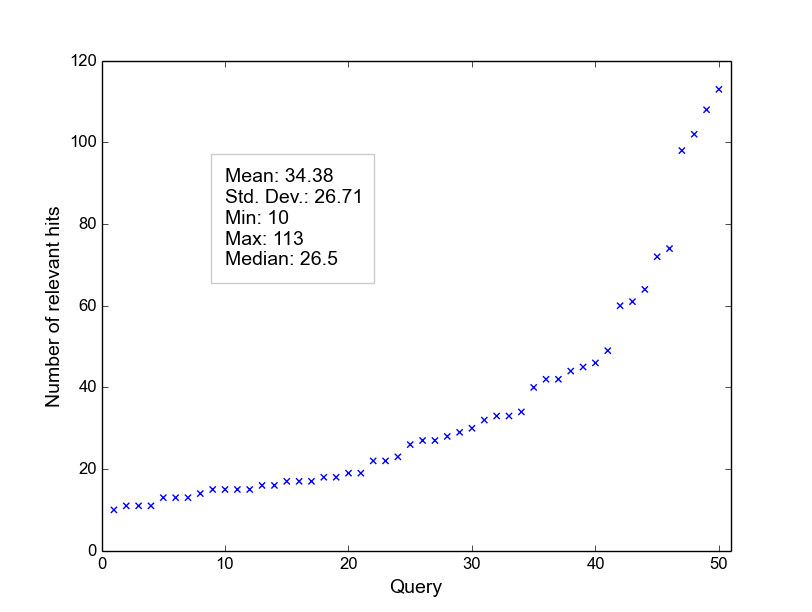
\includegraphics[scale=.4]{reljud.png}
\caption{Number of relevant hits per query in increasing order.}
\label{filter:fig:reljud}
\end{figure}
As we said earlier, % in Section \ref{sec:topicir-filter:video-metadata-collection},
NCRV tags are in-house tags that describe the topics of the fragment with which they are associated.
We consider the NCRV tags as the ground truth about what topics are covered by the fragments.
With this in mind, given a query $q$ and a fragment $f$, we deem $f$ to be topically relevant for $q$ if there is an NCRV tag that is equal with $q$, a synonym of $q$, or a hypernym of $q$. $Y$ is a hypernym of $X$ if every $X$ is a $Y$, for example \textit{canine} is a hypernym of \textit{dog}. Hyperonymy is a transitive relation \cite{wordnet}. More formally, the topical relevance relation is defined as follows
\begin{eqnarray}\label{ground_truth}
Topical\_Relevance &=& \{(q,f)~|~\exists t~(t \in NCRV(f)~\wedge \nonumber\\ 
				  &&(lower(q) = lower(t)~\vee \nonumber\\
				  &&~synonym(lower(q), lower(t))~\vee \nonumber\\
				  &&~hypernym(lower(t), lower(q))))\}
				  \label{top_rel_def}
\end{eqnarray}
where $NCRV(f)$ is the set of all NCRV tags associated with the fragment $f$, $lower(\cdot)$ is the lower case string function, $synonym(w_1, w_2)$ is a binary predicate which is true iff $w_1$ and $w_2$ are synonyms, and $hypernym(w_1, w_2)$ is a binary predicate which is true iff $w_1$ is a hypernym of $w_2$. Figure \ref{filter:fig:reljud} shows the number of relevant fragments in our collection for the queries in the dataset along with additional descriptive statistics. As seen, the median and the average number of relevant hits for a query is approximately 27 and 34, respectively. The lowest number of relevant hits for a query is 10 whereas the highest is 113.

The NCRV tags were primarily created to be used for searching and browsing on the TV-show website by the online community. The tags are displayed prominently on the website's UI which enhances the \textit{social proof} effect \cite{Floeck:social-proof,golder2006usage}, thus many of the tags are incorporated in the terminology of online community. In fact, our chosen query set belongs to the intersection between the NCRV tags and the online community's search terminology as witnessed by Fig. \ref{filter:fig:reljud}. 
As implied by the definition (\ref{top_rel_def}) and seen in Fig. \ref{filter:fig:reljud}, for every query in the query set there is at least one video annotated with the same NCRV tag.
This is sufficient for our narrower aim to determine the relevance for this particular query set and not for \textit{any} query in general. In other words, the mismatch between the NCRV tags and online community's terminology has no impact on the derived relevance judgements for our query set.

Note that while the NCRV tags are currently used by the broadcaster on the TV-show website, there is no guarantee that they, when used as described above, form a complete and accurate ground truth for topical search. We choose this set-up  because the alternative scenario, creating a dedicated topical search ground truth for a limited subset ourselves, would have resulted in a much smaller data set.

We considered variation of definition \ref{ground_truth} where we defined the topical relevance relation only by considering case-insensitive string comparison (omitting synonyms and hyponyms). Even with the modified definition the general conclusions from Sections  \ref{filter:sec:ses} and \ref{sec:topicir-filter:filtering} below remained the same;  while the retrieval metrics of the systems (given by Tables \ref{topicir:table:map-prec-rec} and \ref{filter:table:map-prec-rec}) varied slightly the ordering did not change and the differences remained statistically significant.

\section{Evaluation of Game Tags for Topical Video Search} \label{sec:topicir-filter:all-tags}
In this section we will evaluate the effectiveness of the \textit{Waisda?} tags for topical video search. The results obtained here will serve as a starting point for comparison in the subsequent sections where we will try to improve the retrieval effectiveness of the \textit{Waisda?} tags by filtering those that are irrelevant as topical descriptors.

\subsection{Game tags vs. catalog data}\label{filter:sec:ses}
To address the first research question stated above we created four search engines. Each of them utilizes the same state-of-the-art probabilistic ranking function BM25 and the only variation among them is the metadata they index and use as input for search. Consequently, differences in retrieval performance are attributed solely to the data. We evaluted search engines that index:

\begin{tabular}{lll}
 1. & $SE_{user}$  & all \textit{Waisda?} tags \\
 2. & $SE_{vuser}$& only verified \textit{Waisda?} tags \\
 3. & $SE_{catalog}$&  NCRV catalog data \\
 4. & $SE_{user+catalog}$&  catalog data and all \textit{Waisda?}  tags \\
\end{tabular}

We did not consider using captions for search because we only have them available for a small subset of MBH fragments. If we would have used them in the study, we would have had to settle for much smaller evaluation collection of fragments. Naturally, we did not use the NCRV tags either, since we used them as ground truth for topical relevance.

As said, the combinations of metadata types that are indexed by the various systems are strategically chosen so that the resulting performance metrics from the evaluation dataset will provide answers to the first research question. We compare the performance of $SE_{user}$ against $SE_{catalog}$ to evaluate the performance of the game tags alone when compared to the catalog metadata. By comparing $SE_{user}$ against $SE_{user+catalog}$ we see if the performance of the catalog metadata can be further improved by adding the game tags. Furthermore, we check whether the performance of the game tags can be improved by just using the verified tags ($SE_{user}$ versus $SE_{vuser}$).

\subsection{Results}\label{sec:topicir:results}

\begin{table}[tb]
\centering
\begin{footnotesize}
\begin{tabular}{l|l|l|l}
\toprule
System & MAP & Precision & Recall \\
\hline
$SE_{user}$ & $0.131^{\approx \uparrow}$ & $0.16^{\approx \downarrow}$ & $0.589^{\approx \uparrow}$ \\
\hline
$SE_{vuser}$ & $0.081^{\downarrow \approx}$ & $0.193^{\uparrow \approx}$ & $0.286^{\downarrow \approx}$ \\
\hline
$SE_{catalog}$ & $0.168^{\uparrow \uparrow}$ & $0.438^{\uparrow \uparrow}$ &	$0.291^{\downarrow \uparrow}$ \\
\hline
$SE_{user+catalog}$ & $0.151^{\uparrow \uparrow}$ & $0.17^{\uparrow \downarrow}$ & $0.654^{\uparrow \uparrow}$ \\
\bottomrule
\end{tabular}
\caption{MAP/Precision/Recall scores for the search engines. $\uparrow$, $\downarrow$, and $\approx$ indicate if a score is significantly better, worse, or statistically indistinguishable from the MAP scores of $SE_{user}$ and $SE_{vuser}$, in that order.}
\label{topicir:table:map-prec-rec}
\end{footnotesize}
\end{table}

Table \ref{topicir:table:map-prec-rec} summarizes our findings; the detailed precision and recall metrics for each query can be found in appendix \ref{appen:prec-recall-topical}.
Compared to the previous study (reported in Chapter \ref{chap:ecir}) where we looked at visual relevance, the results for topical relevance are dissapointing. The search performance of game tags ($SE_{user}$) is 28\% below that of the NCRV catalog data ($SE_{catalog}$). Combining the game tags with the catalog metadata does not help either: $SE_{catalog}$ is better than $SE_{user+catalog}$ by 11\%. 
The good news is that $SE_{user}$ outperforms $SE_{catalog}$ on recall: the poor MAP score is largely due to the low precision, only 0.16.

The results are even worse for the verified user tags. While they yield only marginally better search precision, their recall is far worse (see Table \ref{topicir:table:map-prec-rec}). Consequently, $SE_{user}$ outperforms $SE_{vuser}$ by 62\% which suggests that considering all tags is better for topical search than limiting the scope only to verified tags.

In conclusion, the good recall of the game tags does not outweight the low precision. The latter is caused by \textit{Waisda?} tags that match the query but are associated with fragments that are not considered topically relevant. Below, in Section \ref{sec:topicir-filter:filtering}, we attempt to detect and filter out these tags to improve the search performance.

\subsubsection{A Closer Look on Verified Tags}\label{topicir:qual-ana}
The results presented in the previous section suggest that verified tags leave much to be desired when it comes to topical search. To get a better qualitative insight of what happens behind the scenes we carry out an analysis of samples of the results returned by the system that indexes the verified \textit{Waisda?} tags. Our hypothesis is that the tags referring to objects that are visually depicted in the videos are the leading reason for the poor retrieval performance. To test this we analyse a subset of the \textit{false positives} and a subset the \textit{true positives} returned by $SE_{vuser}$. For each query we consider all returned videos--- either true or false positive --- for which captions are available. The subject of the analysis is the tag that caused a given video to be returned for a given query.

First, we classify each tag in the samples into three categories based on the content component --- audio, visual, or both --- it refers to (note that the classification was carried out by a single rater). Tags that refer to concepts that are visually depicted but are not mentioned in the dialog are classified as \textit{only visual}. Tags that are mentioned only in the dialog are classified as \textit{only in captions}. The third category contains the tags that refer to concepts that are both visually depicted and present in the dialog. Second, for each of the categories we compute the average TF-IDF (Term Frequency - Inverse Document Frequency) for the tags in that category. TF-IDF is a numerical statistic which reflects how important a term is to a document in a collection or corpus \cite{tfidf1,tfidf2}. In our context, the TF-IDF score of a tag reflects the relevance of the tag for the associated fragment where the fragments are represented as bags of all tags ascribed to them.  The average TF-IDF score of a category is an indicator of the average relevance of its members relative to the other categories. Lastly, to establish what aspects of the video content the tags from our samples are describing we classify them according to the Panofsky-Shatford model \cite{laurapaper}. This model divides the descriptions into three levels: \textit{general} (generic things in the video), \textit{specific} (specific things), and \textit{abstract} (symbolic things). Each of the levels is further broken down into four facets: \textit{who}, \textit{what}, \textit{where}, and
\textit{when} producing the Panofsky-Shatford 3x4 matrix. There are alternative tag classification schemes \cite{Sigurbjornsson:2008:FTR:1367497.1367542}, however we picked Panofsky-Shatford since it provides insight about the relation of the tag and video content it describes; the role of the concept, denoted by the tag, in the video content is captured by the model, e.g. if the tag \textit{Amsterdam} is classified in \textit{Where Specific} this would signify that this is the location of the scene in the video.

\paragraph{Sampling procedure.}The tags for our analysis are selected as follows.  For each query we consider all returned videos  for which captions are available. The sample of tags consists of all verified tags ascribed to these videos. The reason we restrict only to videos with captions is that in the course of the analysis we check for presence in captions, as described above. The results of the analysis are given in continuation.

\subsubsection{False positives}

\begin{table}[tb]
\centering
\begin{footnotesize}
\begin{tabular}{l|r|r}
\toprule
 & Number & Average TF-IDF\\
 \hline
Only visual & 361 (67\%)& 22.302\\
\hline
Visual and in captions & 19 (3\%)& 55.793\\
\hline
Only in captions  & 161 (30\%)& 49.319\\
\bottomrule
\end{tabular}
\caption{False positives analysis.}
\label{topicir:table:false-pos}
\end{footnotesize}
\end{table}

We start by analysing the false positives returned by the system that indexes the verified tags, $SE_{vuser}$.  The results of the analysis are summarized in Table \ref{topicir:table:false-pos}. The total number of analysed instances is 541. As suspected, the majority of the false positives, about 67\%, are caused by tags referring to concepts that are only visually depicted. Around 30\% of the false positives are caused by tags that appear only in the audio component of the content. The remaining 3\% are caused by tags present both in audio and visual part of the content. Interestingly, it seems that the tags which are present in the audio and refer to a concept that appears visually are less likely to yield false positives. Their presence in both the audio and visual component is a strong indication that they are denoting salient aspects of the content. This is witnessed even more by the fact that this category has the highest average TF-IDF score which measures the importance of a term for a document. In our case the ``document" is the bag of tags associated with the fragment.

\subsubsection{True positives}

\begin{table}[tb]
\centering
\begin{footnotesize}
\begin{tabular}{l|r|r}
\toprule
 & Number & Average TF-IDF\\
 \hline
Only visual & 20 (27\%)& 50.195\\
\hline
Visual and in captions& 33 (45\%)& 96.182\\
\hline
Only in captions  & 21 (28\%)& 60.185\\
\bottomrule
\end{tabular}
\caption{True positives analysis.}
\label{topicir:table:true-pos}
\end{footnotesize}
\end{table}

\begin{table}
\centering
\begin{footnotesize}
\begin{tabular}{l|r|r|r|r|r|r}
\toprule
 & \multicolumn{3}{|c|}{\textbf{True positives}} & \multicolumn{3}{c}{\textbf{False positives}}\\
 \hline
  & \textit{Abstract} & General & Specific & Abstract & General & Specific\\
\hline
Who & & 7& 20& &31 &1\\
\hline
What &4 &34 & &37 & 377&\\
\hline
Where & & 3&6 & &63 &68\\
\hline
When & & & & & &1\\
\bottomrule
\end{tabular}
\caption{Classification of positives.}
\label{topicir:table:pan-shat}
\end{footnotesize}
\end{table}

In this section we continue our analysis with the true positives returned by the system $SE_{vuser}$. The results are summarised in Table \ref{topicir:table:true-pos}. The total number of analysed instances is 74. The figures are following the same trend as the figures for the false positives analysis documented in Table \ref{topicir:table:false-pos}. The tags that are present in the captions and represent concepts depicted visually make the category that yields the highest number of true positives, 45\%. Around 28\% of the true positives are result of tags which are present only in the captions. The remaining 27\% are yielded by tags that denote concepts depicted only visually. Again, the category of tags found both in the audio and visual component have the highest TF-IDF score.

We also classified the positives using the Panofsky-Shatford model \cite{laurapaper}. More precisely, we classified the tags that led to the hit with respect to the returned video fragment. The results from the classification are summarized in Table \ref{topicir:table:pan-shat}. It is interesting to note the disproportionally large number of false positives compared to the number of true positives for the \textit{What} and \textit{Where} facet. In fact, the set of false positives in the \textit{What} facet significantly overlaps with the \textit{only visual} false positives set from Table \ref{topicir:table:false-pos}. For most part these are objects appearing in the foreground and the background of the scenery. The case of the \textit{Where} facet is the more interesting one. The false positives in the \textit{General Where} facet are mostly caused by tags which refer to the dialog in situations where the actors are talking about generic places e.g. their current whereabouts like the \textit{farm}. The false positives in the \textit{Specific Where} facet almost all originate from one query, namely \textit{Amsterdam}. In fact, our collection features a series of videos where a TV crew from Amsterdam travels to other places in the Netherlands and interviews ordinary people. At the beginning of every interview the crew presents themselves at which point they mention that they come from Amsterdam. It is a signature motif in the series and is usually picked up by the players in \textit{Waisda?}. %This suggests that verified tags that refer to \textit{locations} and \textit{objects}\footnote{Most of the tags classified under the \textit{What} facet refer to objects.} are particularly unsuited for topical search. 

After analysing the true and false positives, the general conclusion is that the verified tags usually refer to the more ``obvious", more noticeable, aspects of the content which is in agreement with the conclusions from \cite{DBLP:conf/chi/RobertsonVW09,Jain:2013:GAE:2399187.2399190}. For example, moving objects in the background or in the foreground, prominent stationary objects, or words from dialog are among the things the verified tags denote. This is hardly surprising, after all these are things that are easy to reach consensus on and ultimately that is the goal of the game from the perspective of the players. 

\section{Filtering Non-topical Game Tags}\label{sec:topicir-filter:filtering}

Previously, in Sect. \ref{sec:topicir-filter:all-tags} we investigated how well the tags collected with \textit{Waisda?} are performing with respect to topical search. The general conclusion was that when it comes to using \textit{Waisda?} tags to retrieve fragments that are about a given topic the search performance is  unsatisfactory. This conclusion came with the following caveat: while the search recall is relatively high ($\approx$ 59\%), the search precision is rather low ($\approx$ 16\%). What this means is that a significant portion of topics covered by the fragments are in fact entered as tags by the \textit{Waisda?} players hence the high recall. Moreover, there are also many tags that do not refer to the topics covered by the fragments and when these tags result in a hit the overall search precision goes down. This being said, should the non-topical tags be detected and filtered out from the collection, that would result in increased precision and unchanged recall.
\paragraph{Tag Filters} To make our discussion more precise 	we introduce the notion of a \textit{tag filter}. Speaking formally, a tag filter $F: \mathcal{T}\rightarrow\{true, false\}$ is a unary boolean-valued function defined over the set of all tags, $\mathcal{T}$. For example, we can express the notion of verified tag using tag filters. Indeed, a filter $F_{ver}$ which evaluates to true iff it is passed a verified tag as an argument can be defined in the following way.
\begin{equation*}
F_{ver}(t) = \left\{ 
	\begin{array}{rl}
	true &\mbox{ if $\exists t' \in \mathcal{T}~(t \neq t' \wedge v(t) = v(t') \wedge l(t) = l(t') \wedge $}\\
		& \mbox{~~~~~~~~~~~~~~ $|\tau(t) - \tau(t')| < 10)$} \\
	false &\mbox{ otherwise}
	\end{array}
\right.
\end{equation*}
for every $t \in T$ where $v(\cdot)$ is a function that returns the video fragment the tag passed as an argument is attached to,  $\tau(\cdot)$ is a function that returns the time in seconds relative to the beginning of the video when the tag was entered, and $l(\cdot)$ is a function that returns the label of the tag\footnote{The label of the tag is the actual text entered by the user that contributed the tag.}. Given a video fragment $v \in \mathcal{V}$ and a tag filter $F: \mathcal{T}\rightarrow\{true, false\}$, the set of tags that remain after the filtering is denoted by $Filter:(\mathcal{V} \times \mathcal{T}\rightarrow\{true, false\})\rightarrow \mathcal{P}({T})$ which is defined as follows\footnote{$\mathcal{P}({T})$ denotes the power set of $\mathcal{T}$}

\begin{equation}
Filter(v, F) = \{t |~t \in tags(v), F(t) = true\}
\end{equation}
where $tags(\cdot)$ is a function that returns all tags attached to the fragment passed as an argument.
For instance, $Filter(v, F_{ver})$ denotes the set of all verified tags attached to video fragment $v$.



\subsection{Tag Filters}\label{filter:sec:filters}
In this section we describe the tag filters that are investigated in this study.

\subsubsection{\textit{Entered by at least \textbf{k} Players}}
As seen in Sect. \ref{sec:topicir-filter:all-tags}, considering only verified tags for search results in relatively low search performance. This is mainly due to the fact that verification conditions, as formulated by $F_{ver}$ above, are too restrictive. Consequently, we end up throwing away good tags. Out first try is to relax the conditions by omitting the temporal agreement requirement. Topical tags refer to the entire video, but as our previous studies suggested, the 10 seconds agreement window does not reflect this well as it favours tags that are describing more obvious and short-lived aspects of the content. In particular, we consider the tags that are entered by at least $k$ players where $k\geq2$. More formally, we define the tag filter $F_{play,k}$ as follows
\begin{align}
F_{play,k}(t) = &~|\{p|~p \in \mathcal{P},~\exists t' \in tags(v(t))~(t\neq t' \wedge l(t) = l(t')~\wedge \nonumber\\
			  & ~~~ p(t') = p)\}| \geq k 
\end{align}
for every $t \in \mathcal{T}$ where $\mathcal{P}$ is the set of players, the functions $tags(\cdot)$, $v(\cdot)$ and $l(\cdot)$ are the same as defined above, and the function $p(\cdot)$ returns the player that added the tag passed as an argument. In our experiments, we will vary the value of $k$ in the set $\{2,3,4\}$. Going beyond $k=4$ drastically reduces the number of remaining tags.

\subsubsection{\textit{TF-IDF-rank Take Top k}}
We saw in Sect. \ref{topicir:qual-ana} that the TF-IDF score of a tag is rather indicative as to whether the tag is topical or non-topical. Referring back to Sect. \ref{topicir:qual-ana}, for the analyzed sample of positives, the average TF-IDF score of the true positives was higher than the average TF-IDF score of the false positives. This suggests that the TF-IDF measure favours topical tags. Assuming the correctness of this hypothesis, we exploit this measure to filter out the potentially non-topical game tags.  
In particular, for each fragment in the collection we rank the tags associated with the fragment based on their TF-IDF\footnote{The TF-IDF measure is computed over a corpus of documents. In this particular case the ``documents" are the bag of tags associated with the fragments.} scores in descending order: the tag with the highest TF-IDF score is at the top. Then the filtering is performed by taking only the top $k$ tags for every video. This is expressed by the tag filter $F_{tfidf,k}$ defined as follows
\begin{equation}
F_{tfidf,k}(t) = \left\{ 
	\begin{array}{rl}
	true &\mbox{ if $rank_{tfidf}(t) \leq k$} \\
	false &\mbox{ otherwise}
	\end{array}
\right.
\end{equation}
for every $t \in \mathcal{T}$. The function $rank_{tfidf}: \mathcal{T} \rightarrow \mathbb{N}$ returns the  position (rank) of a given tag $t$ in the ranking in descending order based on TF-IDF score of the tags in the set $tags(v(t))$. As a clarification, given our previous definitions, $tags(v(t))$ denotes the set of tags associated to the fragment $v(t)$ to which the tag $t$ is associated. We vary the value of $k$ in the set $\{5k|~k\in \mathbb{N}, 2 \leq k \leq 20\}$, i.e. all integers from 10 to 100 with increments of 5.

\subsubsection{Latent Dirichlet allocation-based filtering}
Topic models \cite{Hofmann, Blei} are a type of statistical models for discovering abstract `topics' in a collection of documents. One of the most common topic models currently in use is the  Latent Dirichlet Allocation (LDA). The idea behind LDA is to model documents as arising from multiple topics, where a topic is defined to be a probability distribution over a fixed vocabulary of terms --- the set of all unique words in the collection. Specifically, it is assumed that there exists a fixed set of $\mathit{K}$ topics associated with the collection, and that each document exhibits these topics with different proportions. Furthermore, LDA assumes that words are exchangeable within each document, i.e., their order does not affect their probability under the model. In other words, each document is treated as a `bag of words'. We believe that the assumptions underlying the LDA model are valid in and applicable to our context as well. Videos, much like documents, have many layers of meaning and can be viewed as mixture of topics. User tags collected through \textit{Waisda?} can be seen as instantiations of these topics.  The unstructured nature of the tags, --- only weak temporal ordering of tags within video exists, based on the tag entry time --- fits the 'bag of words' metaphor quite well. According to LDA the probability that a tag $t$ appears in video $v$  is given by
\begin{equation}\label{lda-prob-form}
	P(t~|~v) = \sum_{i = 1}^{\mathit{K}}{P(t~|~z_i) P(z_i~|~v)}
\end{equation}
where $P(t~|~z_i)$ is the probability of the tag $t$ for the topic $z_i$ and $P(z_i~|~v)$ is the probability of picking a tag from the topic $z_i$ in $v$ i.e. the proportion of $z_i$ exhibited by $v$. We use the probability  $P(\cdot~|~v)$ given by (\ref{lda-prob-form}) to rank the tags ascribed to $v$ in descending order. The filtering is carried out by taking the top $k$ tags for $v$. This is expressed by the tag filter  $F_{lda,k}$ defined as follows
\begin{equation}
F_{lda,k}(t) = \left\{ 
	\begin{array}{rl}
	true &\mbox{ if $rank_{lda}(t) \leq k$} \\
	false &\mbox{ otherwise}
	\end{array}
\right.
\end{equation}
for every $t \in \mathcal{T}$. The function $rank_{lda}: \mathcal{T} \rightarrow \mathbb{N}$ returns the  position (rank) of a given tag $t$ in the ranking in descending order of the set $tags(v(t))$ based on the probability distribution $P(\cdot~|~v)$ given by (\ref{lda-prob-form}).  We vary the value of $k$ in the set $\{5k|~k\in \mathbb{N},~2 \leq k \leq 20\}$, i.e. all integers from 10 to 100 with increments of 5.


\subsubsection{Player reputation-based filtering}
Another aspect that can be exploited for filtering is the reputation of the players. By incorporating the player's reputation in the tag filtering process we aim to reduce the influence of the `bad' players. According to \cite{Farmer10}, reputation of an entity (e.g. person or an organization) is an opinion about that entity, usually a result of some process of evaluation based on evidence about the entity. In our context, as evidence we consider the events of players ascribing tags to videos which are described by the identity of the player, the tag, the time and the id of the fragment. In fact, this is precisely what is logged by the system and nothing more. A limiting factor is the fact that most of the players ($\approx 99\%$) are anonymous or in other words they only have one recorded session in which they played one or more games. This means that even if the same person played two different sessions as anonymous player there is no way to reliably correlate the sessions. In effect, the amount of evidence we can collect for players is limited.
We define the reputation of a player as the ratio of the number verified tags entered by the player to the number of all tags entered by the player. We consider a verified tag to be a positive evidence for the player's reliability, therefore a higher fraction of verified tags implies higher player's reputation. Instead of computing the ratio directly, we estimate the value by taking the lower bound of Wilson score confidence interval for a Bernoulli parameter \cite{citeulike:1060968,Wilson1927}. The latter approach is more robust in cases where the number of observations (evidence) is small. Now that we have a way to quantify the reputation of the players we define the filtering procedure. The idea is for each tag to combine its TF-IDF score with the reputation of the player that entered it. In particular, for each fragment $v$ we rank the tags in descending order according to the following score
\begin{equation}\label{rep-score}
	score(t) = tfidf(t) \times rep(p(t))
\end{equation}
for each tag $t$ ascribed to $v$ where $tfidf(\cdot)$ is the function that denotes the TF-IDF score and $rep(\cdot)$ returns the reputation for the player $p(t)$ that entered the tag $t$. We see that the score is proportional with the reputation i.e. higher reputation results in higher score.  The filtering is carried out by taking only the top $k$ tags for every video fragment. This is expressed by the tag filter $F_{prep,k}$ defined as follows
\begin{equation}
F_{prep,k}(t) = \left\{ 
	\begin{array}{rl}
	true &\mbox{ if $rank_{score}(t) \leq k$} \\
	false &\mbox{ otherwise}
	\end{array}
\right.
\end{equation}
for every $t \in \mathcal{T}$. The function $rank_{score}: \mathcal{T} \rightarrow \mathbb{N}$ returns the  position (rank) of a given tag $t$ in the ranking in descending order of the set $tags(v(t))$ based on the score function given by (\ref{rep-score}). We vary the value of $k$ in the set $\{5k|~k\in \mathbb{N}, 2 \leq k \leq 20\}$, i.e. all integers from 10 to 100 with increments of 5.

\subsubsection{Network Analysis-based filtering}
Network analysis tools and mechanisms \cite{netan1,netan2} are increasingly used to study folksonomies and social tagging related phenomena \cite{jilung2011network,conf/csse/Wu08b,journals/corr/abs-cs-0509072,Mika:2007:OUU:1229184.1229195,ilprints775,conf/iics/BothorelB11}. The crux of these approaches is to  represent the domain knowledge as a network (graph) and apply network analysis tools to investigate the phenomenon of interest. In our particular case, we exploit network analysis to detect and filter out non-topical tags. The general idea is to build a network for each video fragment that captures the semantic connectedness among the tags associated with that fragment. Once the network is build we exploit network centrality measures to rank the tags according to their importance. The intuition is the more central a given tag is the higher its connectedness with the other tags is and therefore that tag has higher importance as content descriptor. We consider three centrality measures: pagerank, weighted degree centrality and eigenvector centrality. However these methods did not perform as well as TF-IDF and LDA and for space reasons we omit them from our discussion.  

\subsection{Search Engines}
As said, our goal is to investigate various ways how the non-topical tags can be detected and filtered out with the ultimate goal of improving search performance. To this end, we define a number of tag filters and apply them to every fragment in the collection in the manner described above. Each tag filter yields a filtered collection of tags which is used as an input for search by systems (search engines). Note that there are two systems per tag filter: one that indexes \textit{only} the filtered collection of tags and one that indexes \textit{both} the filtered collection of tags \textit{and} the catalog metadata. The structure of all systems is identical: each system uses the same state-of-the-art probabilistic ranking function BM25, but indexes different metadata for search, depending on the tag filter and whether or not catalog data is considered. Thus, the only variations among the systems is the input that they exploit for search\footnote{Again, we built the systems using the Xapian open source search engine library and did not vary the parameters for the BM25 function but used the defaults provided by Xapian.}.

\subsection{Results} \label{filter:sec:res}

\begin{table}[tb]
\centering
\begin{footnotesize}
\begin{tabular}{l|l|l|l|l}
\toprule
\multirow{5}{*}{\textbf{Baseline}} & \textbf{System} & \textbf{MAP} & \textbf{Precision}& \textbf{Recall}\\
	\hline
&$SE_{catalog}$ & $0.168^{\approx\uparrow \uparrow}$ & $0.438^{\approx\uparrow \uparrow}$ &	$0.291^{\approx\downarrow \uparrow}$ \\
\cline{2-5}
&$SE_{user}$ & $0.131^{\downarrow\approx \uparrow}$ & $0.16^{\downarrow \approx \downarrow}$ & $0.589^{\uparrow\approx \uparrow}$ \\
\cline{2-5}
&$SE_{vuser}$ & $0.081^{\downarrow \downarrow \approx}$ & $0.193^{\downarrow \uparrow \approx}$ & $0.286^{\downarrow\downarrow \approx}$ \\
\hline
\multirow{8}{*}{\textbf{Tag filters}} &$SE_{F_{tfidf,80}}$ & $0.171^{\uparrow\uparrow\uparrow}$ & $0.221^{\downarrow\uparrow\uparrow}$ & $0.523^{\uparrow\downarrow\uparrow}$ \\
\cline{2-5}
& $SE_{F_{lda,30}}$ & $0.149^{\downarrow\uparrow\uparrow}$ & $0.22^{\downarrow\uparrow\uparrow}$ & $0.454^{\uparrow\downarrow\uparrow}$ \\
\cline{2-5}
%&$S_{F_{wdeg,80}}$ & $0.156$ & $0.197$ & $0.56$ \\
%\cline{2-5}
%&$S_{F_{pagerank,80}}$ & $0.155$ & $0.196$ & $0.559$ \\
%\cline{2-5}
&$SE_{F_{prep,70}}$ & $0.145^{\downarrow\uparrow\uparrow}$& $0.215^{\downarrow\uparrow\uparrow}$& $0.404^{\uparrow\downarrow\uparrow}$\\
\cline{2-5}
%&$SE_{F_{rep,2}}$ & $0.103$ & $0.206$ & $0.364$ \\
%\cline{2-5}
&$SE_{F_{play,2}}$ & $0.083^{\downarrow\downarrow\approx}$ & $0.198^{\downarrow\uparrow\approx}$ & $0.287^{\downarrow\downarrow\approx}$ \\
\cline{2-5}
&$SE_{F_{tfidf,80 + catalog}}$ & $0.199^{\uparrow\uparrow\uparrow}$ & $0.233^{\downarrow\uparrow\uparrow}$ & $0.603^{\uparrow\uparrow\uparrow}$ \\
\cline{2-5}
&$SE_{F_{lda,30 + catalog}}$ & $0.174^{\uparrow\uparrow\uparrow}$ & $0.258^{\downarrow\uparrow\uparrow}$ & $0.53^{\uparrow\downarrow\uparrow}$ \\
\cline{2-5}
&$SE_{F_{prep,70 + catalog}}$ & $0.19^{\uparrow\uparrow\uparrow}$ & $0.243^{\downarrow\uparrow\uparrow}$ & $0.541^{\uparrow\downarrow\uparrow}$ \\
\cline{2-5}
&$SE_{F_{play,2 + catalog}}$ & $0.15^{\downarrow\uparrow\uparrow}$ & $0.247^{\downarrow\uparrow\uparrow}$ & $0.449^{\uparrow\downarrow\uparrow}$\\
\bottomrule
\end{tabular}
\caption{MAP/Precision/Recall scores for the search engines. Notational convention: the system that indexes the data obtained by applying the filter $F$ is denoted by $SE_F$; only the best performing filters for each filtering approach are shown. $\uparrow$, $\downarrow$, and $\approx$ indicate if a score is significantly better, worse, or statistically indistinguishable from the scores of $SE_{catalog}$, $SE_{user}$, and $SE_{vuser}$, respectively.}
\label{filter:table:map-prec-rec}
\end{footnotesize}
\end{table}

In this section we present the results of running the search engines that index the filtered collection of tags using the tag filters described in Sect. \ref{filter:sec:filters} against the evaluation dataset. The evaluation metrics are summarized in Table \ref{filter:table:map-prec-rec}. For reference we copied the metrics for the systems $SE_{user}$, $SE_{vuser}$, and $SE_{catalog}$ from Sect. \ref{sec:topicir:results}. We use the following notational convention in the table: the system that indexes the data obtained by applying the filter $F$ is denoted by $SE_F$ and the system that indexes the data obtained by applying the filter $F$ and the catalog data is denoted by $SE_{F+catalog}$. The system that we are trying to beat is $SE_{catalog}$ since it is the best performing one and an approximation of the present search functionality.

\subsubsection{\textit{Entered by at least \textbf{k} Players}}
We start off by presenting the results for the system $SE_{F_{play,k}}$ which indexes all the tags that are entered by at least $k$ different players. As said before, we varied the value of $k$ in the set $\{2,3,4\}$ and as the value of $k$ increased the precision, recall, and MAP score monotonically decreased. The statistics for the best performing system $SE_{F_{play,2}}$ are presented in Table \ref{filter:table:map-prec-rec}. As we can see, $SE_{F_{play,2}}$ performs only marginally better than the system that indexes the verified tags,  $SE_{vuser}$, and much worse compared to the system that indexes all tags, $SE_{user}$. It seems $F_{play,2}$ is able to detect only a small fraction of the good tags that are outside of the set of verified tags, hence the marginal increase in precision and recall.
The combination of the tag filtering and catalog metadata worsens the matters. $SE_{F_{play,2 + catalog}}$ has higher recall than $SE_{catalog}$ but comparatively lower precision which results in lower MAP score.


\subsubsection{Latent Dirichlet allocation-based filtering}
This section presents the results for the system $S_{F_{lda,30}}$ which indexes only the top $k$ tags from each fragment where the ranking is based on the a posteriori probability that a given tag is assigned to the fragment as estimated by the LDA model. The value of $k$ was varied from 10 to 100 with an increment of 5. The best results are achieved for $k=30$ and are shown in Table \ref{filter:table:map-prec-rec}. As we can see, $S_{F_{lda,30}}$ outperforms that system $SE_{user}$ that indexes all user tags by 14\%. However, the retrieval performance of $S_{F_{lda,30}}$ falls short when compared with the systems $SE_{catalog}$ and $S_{F_{tfidf,80}}$ which outperform it by 28\% and 31\%, respectively.
The combination of the catalog data and LDA tag filtering yields only a marginal improvement in performance: $SE_{F_{lda,30 + catalog}}$ outperforms $SE_{F+catalog}$ only by $3\%$ with respect to the MAP score.
\paragraph{Discussion} A potential explanation for the poor performance of the LDA based filtering is the size of the corpus. Our tag/fragment collection is not large enough for the LDA model to provide a good estimation of the underlying topic structure. In fact, this was our suspicion all along however we decided to include LDA for the sake of completeness --- since TF-IDF and LDA are among the most commonly used methods for measuring word to document relevance and topic inference.


\subsubsection{Player reputation-based filtering}

\begin{figure}
\centering
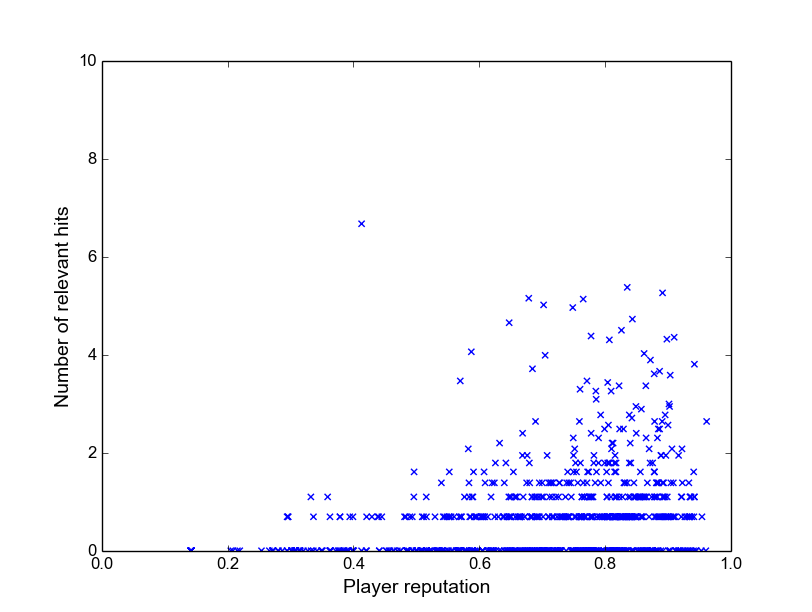
\includegraphics[scale=.4]{filterrepcorr}
\caption{Correlation between the reputation and the number of relevant hits for the players. The horizontal axis displays the reputation of the player in increasing order and the vertical axis shows the number of relevant videos retrieved using a tag entered by the corresponding player.}
\label{filter:fig:repcorr}
\end{figure}

This section outlines the results for the system $S_{F_{prep,k}}$ which takes only the top $k$ tags for each fragment where the ranking is based on the combination of the TF-IDF score and the reputation of the players.
As previously, the value of $k$ was varied from 10 to 100 with an increment of 5.
The best results are achieved for $k=70$ and are displayed in Table \ref{filter:table:map-prec-rec}. As we can see there is a an improvement of $11\%$ with respect to the MAP score compared to the system $SE_{user}$ which indexes all user tags. However, the search performance of  $S_{F_{prep,70}}$ is worse for all three metrics than the system $S_{F_{tfidf,80}}$ which ranks and filters the tags based only on their TF-IDF scores. This means that considering the reputations of the players in combination with the TF-IDF ranking in this case only worsened the matters for the TF-IDF based filtering. This conclusion is further supported by the fact that $SE_{tfidf,80 + catalog}$ outperforms  $SE_{prep,70 + catalog}$ by $5\%$ with respect to the MAP score. 
\paragraph{Discussion} Figure \ref{filter:fig:repcorr} shows the correlation between the reputation of the players and their success in providing tags that resulted in relevant search results. In particular, the horizontal axis shows the reputation for each of the users in increasing order whereas the vertical axis presents the number of relevant video fragments that can be retrieved using tags entered by the corresponding player. As seen, higher reputation does not entail higher success rate. In fact, many of the most  reputable players are among the ones that were the least successful. This means that computing reputation in the manner outlined above may not be the best predictor for the ability of the player to provide topically relevant tags. 
Moreover, considering \cite{DBLP:conf/chi/RobertsonVW09,Jain:2013:GAE:2399187.2399190} our reputation estimation method assigns higher reputation to players which settle on low-effort tags. Consequently, tags favored by this filtering method will tend to be more `obvious'.
Alternative explanation is that there is not sufficient data available to reliably estimate the reputation of the players. Recall that 99\% of the players are registered as anonymous and the only data available for them is a single session of playing \textit{Waisda?}. 

\subsubsection{\textit{\textit{TF-IDF-rank Take Top k}}}

\begin{figure}
\centering
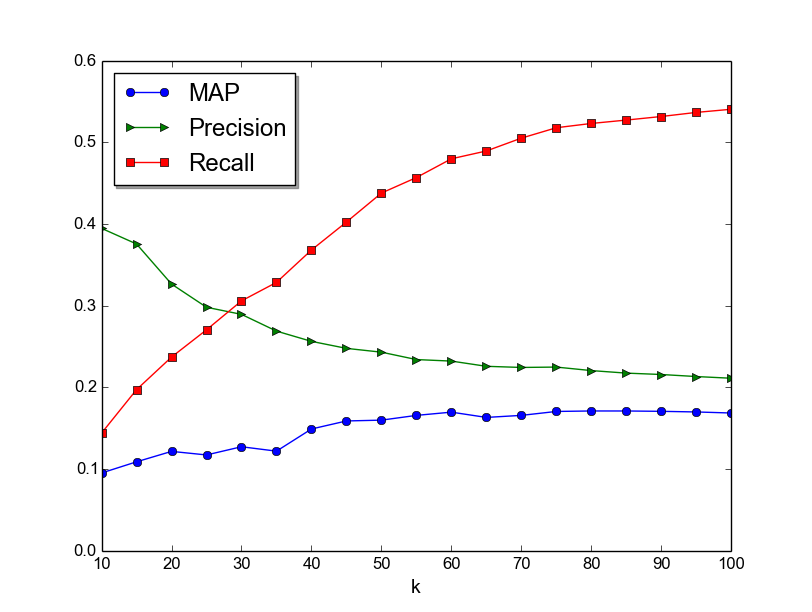
\includegraphics[scale=.4]{tfidfmets}
\caption{Search performance statistics for the systems $SE_{F_{tfidf,k}}$.}
\label{filter:fig:tfidfstats}
\end{figure}

This section outlines the results for the systems $S_{F_{tfidf,k}}$ which consider only the top $k$ tags for each fragment where the ranking is based on the TF-IDF scores of the tags. We vary the value of $k$ from 10 to 100 with increments of 5. Figure \ref{filter:fig:tfidfstats} presents the search performance statistics as the value of $k$ varies. Not surprisingly, as the value of $k$ increases the search precision and the search recall decrease and increase, respectively. Moreover, the MAP score steadily increases until $k$ equals 80, where the maximal value is reached, and then it starts to decrease. As shown in Table \ref{filter:table:map-prec-rec}, the MAP score of $S_{F_{tfidf,80}}$ is $0.171$ which means it significantly outperforms $SE_{user}$, the systems that indexes all user tags. Indeed, the increase in search performance is 31\%. What is more important is that $S_{F_{tfidf,80}}$ slightly outperforms even $SE_{catalog}$, which until now was the best performing one and the system that we are trying to beat. This suggests that TF-IDF score is indeed a good indication of the quality of the tags as topical descriptors and can be used to filter out the non-topical tags. Furthermore, the combination of catalog metadata and TF-IDF filtering proves to be beneficial: $SE_{tfidf,80 + catalog}$ outperforms  $SE_{catalog}$ by $18\%$. The improvement is caused by the fact that the TF-IDF ranked tags increase the search recall of the catalog metadata by factor of $2$; the recall of $SE_{tfidf,80 + catalog}$ is higher than the recall of $SE_{catalog}$ by $107\%$.

\section{Conclusion and Discussion}\label{sec:topicir-filter:con}
In this paper we studied to what extend players enter tags which are valid topical descriptors of the video material. Another aim was to derive insights about players’ tagging practices that are associated with ascribing topical tags. The study was carried out with the focus on topical search.

In Section \ref{sec:topicir-filter:all-tags} we evaluated the search performance of the entire unprocessed collection of the user tags. The general conclusion is that the search performance of the raw, unprocessed, user tags for retrieving videos based on topic leaves much to be desired. While the search recall of the user tags is relatively satisfactory the precision is rather poor. Our analysis showed that a significant portion of the topics are indeed captured by the user tags. However, there are also many user tags that do not pertain to the subject (\textit{semantics}) of the video, but refer to the more \textit{syntactic} aspects such as what is \textit{seen} or \textit{heard}. It is the latter group that is responsible for the false positives and thereby hurting the search precision. Therefore, if user tags are to be used for topical search, a preprocessing step is required that will identify and filter out the non-topical user tags.

The quality of the tags as topical descriptions was addressed in Section \ref{sec:topicir-filter:filtering} where we looked into several ways we can detect and filter out the non-topical user tags. While the different methods that we studied performed with various success, the conclusion is that the game tags can be successfully exploited for topical video search provided there is a filtering process that would reduce or eliminate the effect of the non-topical tags. Our results show that after TF-IDF-based filtering game tags can emulate the retrieval performance of the best performing system that utilizes manually crafted metadata for search. Moreover, combining TF-IDF filtered game tags with the manually crafted metadata  yields an improvement of retrieval performance by $18\%$. The improvement is attributed to the increased retrieval recall stemming from the game tags. An important consequence of this result is that tagging games provide a cost-effective alternative for AV collection owners that do not possess the required manpower to manually annotate their material.

Successfully deploying a GWAP is no small feat. Atracting new players and keeping them engaged over time is vital for success and requires continuous publicising efforts. The experience gained from the \textit{Waisda?} project showed that targeting the fanbase of the TV series being tagged in the game is an effective method of attracting new players. Player’s engagement can be sustained with in-game motivational mechanisms such as leaderboards, and with time-limited contests offering awards for the top performers. Planning and executing such activities is costly, however the cost is independent of the size of the video collection.  The cost of manual annotation, on the other hand, increases linearly with the size of the collection and will eventually outweigh the \textit{Waisda?}-related costs.

What makes video annotation a difficult task is the fact that video is a medium that is extremely rich in meaning. The taggers can get overwhelmed by the complex interplay of objects and events especially in the fast-paced game setting. Our qualitative analysis showed that significant portion of the \textit{Waisda?}
tags refer to more noticeable aspects of the content such as moving objects in the background or in the foreground, or prominent stationary objects. This is hardly surprising, after all these are things that are easy to reach consensus on and ultimately that is the goal of the game from the perspective of the players. We also observed that the tags which are present in the audio and refer to a concept that appears visually are more likely to be topical descriptors. Their presence in both the audio and visual component is an indication that they are denoting salient aspects of the content. Therefore, if the goal of the AV collection owners is collecting topical tags, this insight can be operationalized in the game by instructing the players to tag things that are both on screen and in the audio.

\textit{Waisda?} is a production grade open-source crowd-sourcing tool which is relatively easy to set-up and after the suitable processing the collected tags can be exploited for retrieval. We believe that this is an important step toward making the AV heritage more accessible on the Web and in general making the Web more connected.
